% Mechanistic Interpretability of Portuguese in Multilingual LLMs
% BRACIS 2026 — Springer LNAI format, double-anonymous
%
\documentclass[runningheads]{llncs}

\usepackage[T1]{fontenc}
\usepackage{graphicx}
\usepackage{booktabs}
\usepackage{amsmath}
\usepackage{amssymb}
\usepackage{multirow}
\usepackage{xcolor}
\usepackage{subcaption}
\usepackage[hidelinks]{hyperref}
\renewcommand\UrlFont{\color{blue}\rmfamily}
\urlstyle{rm}

\begin{document}

\title{Cross-Family Mechanistic Interpretability of Portuguese\\Representation in Multilingual LLMs via Sparse Autoencoders}

\titlerunning{Cross-Family Mechanistic Interpretability of Portuguese in LLMs}

% Double-anonymous: no author info
\author{Anonymous Author(s)}
\authorrunning{Anonymous}
\institute{Anonymous Institution}

\maketitle

% ============================================================
\begin{abstract}
How multilingual language models internally represent individual languages remains poorly understood, yet this question matters for generation quality, bias diagnosis, and controllable generation. We investigate how two model families, Gemma-2-2B and Llama~3.1~8B, represent Portuguese by using Sparse Autoencoders (SAEs) to decompose residual stream activations into interpretable features. We train 16 custom SAEs (ReLU+L1 and TopK architectures) and use pretrained SAEs (Gemma Scope and Llama-Scope) to catalog Portuguese-specific features across multiple layers in both models. Causal steering experiments reveal a qualitative difference between model families: suppressing Portuguese features in Gemma~2B redirects generation to Spanish/Catalan, while in Llama~8B it redirects to English, suggesting different internal language organizations that we term the Romance-language continuum and English substrate models. Progressive multi-layer steering shows that language identity is encoded in mid-to-late layers (15--25), with a monolinguality analysis confirming sharper language boundaries in Llama (0.270) than Gemma (0.252). Pairwise similarity analysis reveals that typological distance is encoded from the earliest layers, with finer Romance-language distinctions emerging progressively in deeper layers. To our knowledge, this is the first cross-family mechanistic analysis of Portuguese representation in LLMs.

\keywords{Mechanistic Interpretability \and Sparse Autoencoders \and Multilingual LLMs \and Portuguese NLP \and Feature Steering}
\end{abstract}

% ============================================================
\section{Introduction}
\label{sec:intro}

Modern large language models (LLMs) process dozens of languages simultaneously, yet little is known about how they internally represent each one. This gap has practical consequences: improving generation quality in under-represented languages, diagnosing linguistic biases, and building control mechanisms all depend on understanding the internal geometry of multilingual representations.

Sparse Autoencoders (SAEs) decompose dense neural activations into sparse, interpretable features~\cite{bricken2023monosemanticity,cunningham2023sparse} and have become a standard tool in mechanistic interpretability. Pretrained SAE suites now exist for several model families, including Gemma Scope~\cite{lieberum2024gemma} and Llama-Scope~\cite{he2024llama}. Existing analyses focus primarily on English-language phenomena, however, leaving open the question of how SAEs can reveal language-specific representations in multilingual settings.

We address this gap with a cross-family mechanistic interpretability study focused on Portuguese, a language spoken by over 250 million people and present in varying proportions across LLM training corpora. Our analysis spans two model families, Gemma-2-2B (26 layers, $d_\text{model}=2{,}304$) and Llama~3.1~8B (32 layers, $d_\text{model}=4{,}096$), chosen for their architectural differences, distinct training data compositions, and the availability of pretrained SAE suites. We employ both pretrained and custom-trained SAEs.

We make three contributions. First, suppressing Portuguese-specific SAE features produces qualitatively different fallback behaviors (Spanish/Catalan in Gemma vs.\ English in Llama), revealing two internal organizations that we term the ``Romance-language continuum'' and ``English substrate'' models. Second, amplifying Portuguese features forces Portuguese output from non-Portuguese prompts while suppressing them causes language switching, establishing a causal rather than correlational link between features and language generation. Third, TopK SAE reconstruction varies across base models (79.7\% FVE on Gemma vs.\ 98.0\% on Llama) while ReLU+L1 exceeds 99\% on both, showing that architecture ranking does not transfer automatically across base models.

% ============================================================
\section{Related Work}
\label{sec:related}

\paragraph{Mechanistic Interpretability with SAEs.}
Sparse autoencoders decompose neural activations into overcomplete, sparse representations where individual features can be more interpretable than individual neurons~\cite{cunningham2023sparse,bricken2023monosemanticity}; Gao et al.~\cite{gao2024scaling} scaled SAE training and proposed standard metrics (Fraction of Variance Explained, dead-feature ratios), and Deng et al.~\cite{deng2025survey} survey the area. SAEBench~\cite{karvonen2025saebench} and AxBench~\cite{wu2025axbench} caution that proxy metrics do not reliably predict downstream utility and that simple baselines can outperform SAEs for behavioral steering, though SAEs retain advantages for mechanistic and feature-level analysis, which is our focus. Bricken et al.~\cite{bricken2023monosemanticity} introduced clamping SAE features as a causal intervention, which we extend to the multilingual setting. Pretrained SAE suites exist for Gemma~\cite{lieberum2024gemma} (16k features, ReLU) and Llama~\cite{he2024llama} (32k features, JumpReLU).

\paragraph{Multilingual Representations in LLMs.}
Wendler et al.~\cite{wendler2024llamas} showed that Llama~2 uses English as an internal \emph{lingua franca}, and Tang et al.~\cite{tang2024language} identified language-specific neurons in multilingual transformers. Most directly relevant, Deng et al.~\cite{deng2025unveiling} concurrently proposed a monolinguality metric for SAE features and showed that ablating language-specific features selectively impacts single-language performance. Our work differs by comparing across model families (Gemma vs.\ Llama) rather than within one family, focusing on Portuguese (an under-studied language in interpretability research), and directly comparing SAE architectures (ReLU+L1 vs.\ TopK) across models.

\paragraph{Portuguese Language Processing.}
Prior work on Portuguese NLP includes BERTimbau~\cite{souza2020bertimbau} and multilingual models fine-tuned for Portuguese tasks, but these target downstream performance rather than internal mechanisms. Our study provides the first systematic catalog of Portuguese-specific features discovered through SAE decomposition, with causal validation via steering.

\paragraph{Concurrent Work on Language Steering.}
Several concurrent works also apply SAEs to multilingual steering: LangFIR~\cite{langfir2026} identifies language-specific features from monolingual data via random-token filtering; SASFT~\cite{sasft2026} diagnoses code-switching and mitigates it via SAE-guided finetuning; Causal Language Control~\cite{causal_lang_control2025} achieves 90\% single-feature steering success in Gemma-2B. These works target typologically distant pairs (EN$\to$ZH, EN$\to$JA); our study targets Romance languages, where steering is harder due to shared representations.

% ============================================================
\section{Methodology}
\label{sec:method}

\subsection{Models and Data}

We analyze two model families (Table~\ref{tab:models}), chosen for their architectural differences and availability of pretrained SAEs.

\begin{table}[t]
\centering
\caption{Base models and pretrained SAEs used in this study.}
\label{tab:models}
\begin{tabular}{lccccl}
\toprule
\textbf{Model} & \textbf{Params} & \textbf{Layers} & $d_\text{model}$ & \textbf{SAE $d_\text{sae}$} & \textbf{SAE Activation} \\
\midrule
Gemma-2-2B & 2B & 26 & 2,304 & 16,384 & ReLU \\
Llama 3.1 8B & 8B & 32 & 4,096 & 32,768 & JumpReLU \\
\bottomrule
\end{tabular}
\end{table}

For multilingual evaluation we use FLORES-200~\cite{costa2022no} parallel sentences in five languages (PT, EN, ES, FR, IT), 1,012 pairs per language; because the sentences are parallel translations, differential activation patterns reflect linguistic rather than semantic differences. SAE training data comes from Portuguese Wikipedia ($\sim$2M tokens per model), tokenized with each model's native tokenizer (SentencePiece for Llama, BPE for Gemma); residual stream activations are extracted with TransformerLens~\cite{nanda2022transformerlens} and stored as float16 tensors. We also analyze Gemma-2-9B (42 layers, $d_\text{model}{=}3{,}584$) for within-family cross-scale comparison, using raw neuron activations since Gemma Scope SAEs were not available for the 9B model at the time of this study.

\subsection{Sparse Autoencoder Architectures}

We compare two SAE architectures, each trained on layer-10 residual stream activations from Portuguese Wikipedia:

\paragraph{ReLU+L1.} The encoder maps an input activation $\mathbf{x} \in \mathbb{R}^{d}$ to a sparse code $\mathbf{f} = \text{ReLU}(W_\text{enc}(\mathbf{x} - \mathbf{b}_\text{pre}) + \mathbf{b}_\text{enc}) \in \mathbb{R}^{d_\text{sae}}$, which the decoder reconstructs as $\hat{\mathbf{x}} = W_\text{dec}\mathbf{f}$. Training minimizes:
\begin{equation}
\mathcal{L}_{\text{ReLU}} = \|\mathbf{x} - \hat{\mathbf{x}}\|_2^2 + \lambda \|\mathbf{f}\|_1
\label{eq:relu_loss}
\end{equation}
with decoder columns normalized to unit norm at each step.

\paragraph{TopK.} Same encoder-decoder architecture, but enforces exact sparsity by retaining only the top-$k$ encoder activations (applying ReLU to them) and zeroing the rest. The loss is MSE only:
\begin{equation}
\mathcal{L}_{\text{TopK}} = \|\mathbf{x} - \hat{\mathbf{x}}\|_2^2
\label{eq:topk_loss}
\end{equation}
since sparsity (the $\ell_0$-norm $\|\mathbf{f}\|_0 = k$ exactly) is enforced structurally rather than via penalty. We use $L_0$ throughout to refer to this $\ell_0$-norm sparsity count.

For each base model we train 8 SAE configurations (totaling 16 custom SAEs): both architectures at $d_\text{sae}\in\{4{,}096, 16{,}384\}$, with $\lambda\in\{5\times 10^{-4}, 10^{-4}\}$ for ReLU+L1 and $k\in\{32, 64\}$ for TopK. Training uses Adam (lr $3 \times 10^{-4}$) for 1 epoch with batch size 4,096 (Gemma) or 2,048 (Llama).

\subsection{Differential Feature Analysis}
\label{sec:differential}

To identify Portuguese-specific features, we compute a differential activation score. For each SAE feature $i$, we first compute the mean activation $\bar{a}_i^{l}$ across all FLORES tokens in language $l$. The differential activation score is:
\begin{equation}
s_i = \frac{\bar{a}_i^{\text{PT}} - \frac{1}{|\mathcal{L}'|}\sum_{l \in \mathcal{L}'}\bar{a}_i^{l}}{\sigma_i}
\label{eq:diff}
\end{equation}
where $\mathcal{L}' = \{\text{EN, ES, FR, IT}\}$ is the set of contrast languages, $\mathcal{L} = \mathcal{L}' \cup \{\text{PT}\}$ is the full set of five FLORES languages, and $\sigma_i = \text{std}(\{\bar{a}_i^{l}\}_{l \in \mathcal{L}})$ normalizes by cross-language variability. Features with $s_i > 2$ are considered \emph{strongly Portuguese-specific}: their Portuguese activation is more than 2 standard deviations above the cross-language mean.

We apply this analysis at 6 layers per model: layers 0, 5, 10, 15, 20, 25 for Gemma~2B; layers 0, 5, 10, 16, 21, 26 for Llama~8B (selected at approximately equivalent relative positions).

\subsection{Monolinguality Metric}
\label{sec:monolinguality}

To compare how sharply languages separate inside each model, we compute a monolinguality metric on raw residual-stream neurons (not SAE features). We operate on raw neurons so that the same procedure can be applied to Gemma-2-9B in the cross-scale analysis of Section~\ref{sec:crossscale}, where no pretrained SAE suite is available. For each neuron $i$ and language $L$, let $a_i(L) = |\overline{x_i^{(L)}}|$ denote the absolute mean activation of neuron $i$ on FLORES sentences of language $L$, where the inner mean is taken first over tokens and then over sentences. A neuron is \emph{PT-dominant} at a given layer if $\arg\max_{L \in \mathcal{L}} a_i(L) = \text{PT}$, i.e., its absolute activation is largest on Portuguese among the five FLORES languages. For each PT-dominant neuron, its monolinguality is
\begin{equation}
m_i(\text{PT}) = \frac{a_i(\text{PT})}{\sum_{L \in \mathcal{L}} a_i(L)},
\qquad \mathcal{L} = \{\text{PT, EN, ES, FR, IT}\}.
\label{eq:monolinguality}
\end{equation}
Values close to $1/|\mathcal{L}| = 0.2$ indicate a neuron that activates comparably across all languages; values near $1$ indicate a neuron that fires almost exclusively on Portuguese. We report, per model, the mean of $m_i(\text{PT})$ over PT-dominant neurons at each analyzed layer, and a single per-model figure obtained by averaging across those layers.

\subsection{Steering Experiments}

We perform causal interventions by hooking into the model's forward pass at layer 10 and modifying SAE-encoded features:

\paragraph{Amplification.} We encode the residual activation through the SAE, multiply the top-20 Portuguese-specific features by factor $\alpha \in \{1, 2, 5, 10\}$, decode back, and replace the original activation. This tests whether increasing PT feature magnitudes forces Portuguese generation.

\paragraph{Suppression.} Same procedure, but the top-20 Portuguese features are set to zero. This tests whether removing PT features causes language switching and, in particular, which language the model defaults to.

For Gemma~2B we use Gemma Scope (layer 10, 16k features); for Llama~8B we use Llama-Scope (layer 10, 32k features, JumpReLU). We test on 10 prompts per language (PT, EN, ES, FR), generating 50 tokens with temperature 0.7.

% ============================================================
\section{Experiments and Results}
\label{sec:results}

\subsection{Reconstruction Quality}
\label{sec:reconstruction}

Table~\ref{tab:reconstruction} reports the best configuration per architecture for each model; Figure~\ref{fig:pareto} shows the full Pareto frontier across all 16 custom SAEs.

\begin{table}[t]
\centering
\caption{Best SAE per architecture per model (evaluated on FLORES PT activations, layer 10). FVE = Fraction of Variance Explained. $L_0$ = mean number of non-zero features per activation ($\ell_0$-norm). Dead = fraction of features never activated.}
\label{tab:reconstruction}
\begin{tabular}{llrrrr}
\toprule
\textbf{Model} & \textbf{Architecture} & \textbf{FVE (\%)} & \textbf{$L_0$} & \textbf{MSE} & \textbf{Dead (\%)} \\
\midrule
\multirow{2}{*}{Gemma 2B} & ReLU+L1 ($d$=4k, $\lambda$=1e-4) & 99.19 & 4,040 & 0.063 & 0.0 \\
 & TopK ($d$=16k, $k$=64) & 79.65 & 64 & 1.578 & 35.3 \\
\midrule
\multirow{2}{*}{Llama 8B} & ReLU+L1 ($d$=16k, $\lambda$=1e-4) & \textbf{99.83} & 7,684 & 0.001 & 1.1 \\
 & TopK ($d$=16k, $k$=64) & 98.01 & 64 & 0.009 & 31.3 \\
\bottomrule
\end{tabular}
\end{table}

\begin{figure}[t]
\centering
\begin{subfigure}[b]{0.48\textwidth}
    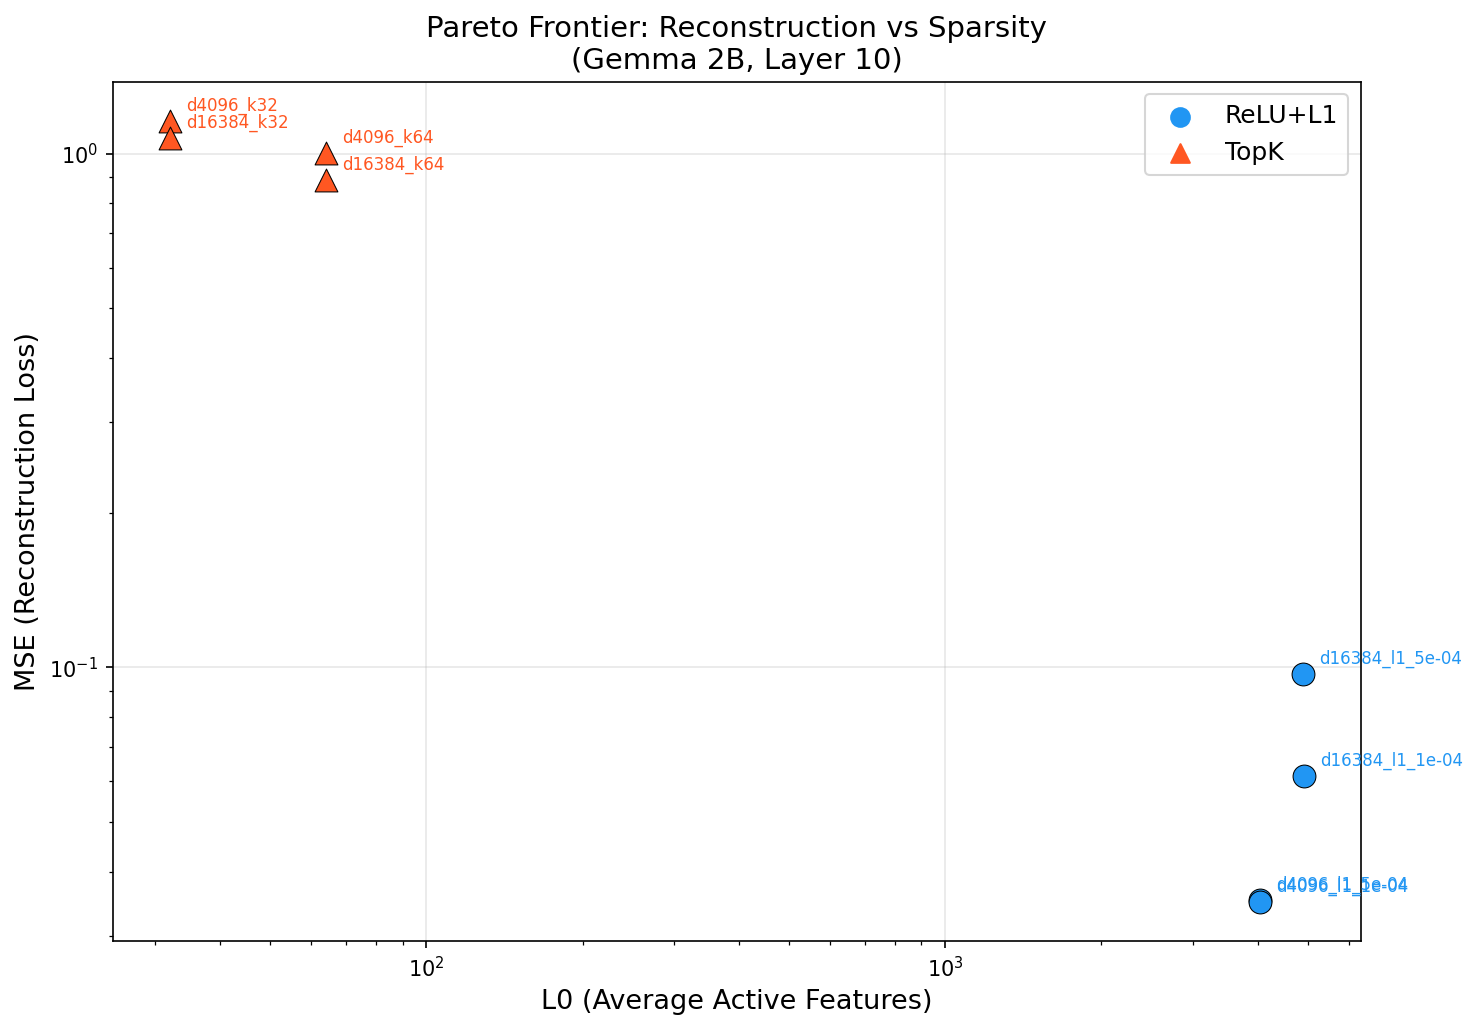
\includegraphics[width=\textwidth]{figures/pareto_gemma.png}
    \caption{Gemma 2B}
\end{subfigure}
\hfill
\begin{subfigure}[b]{0.48\textwidth}
    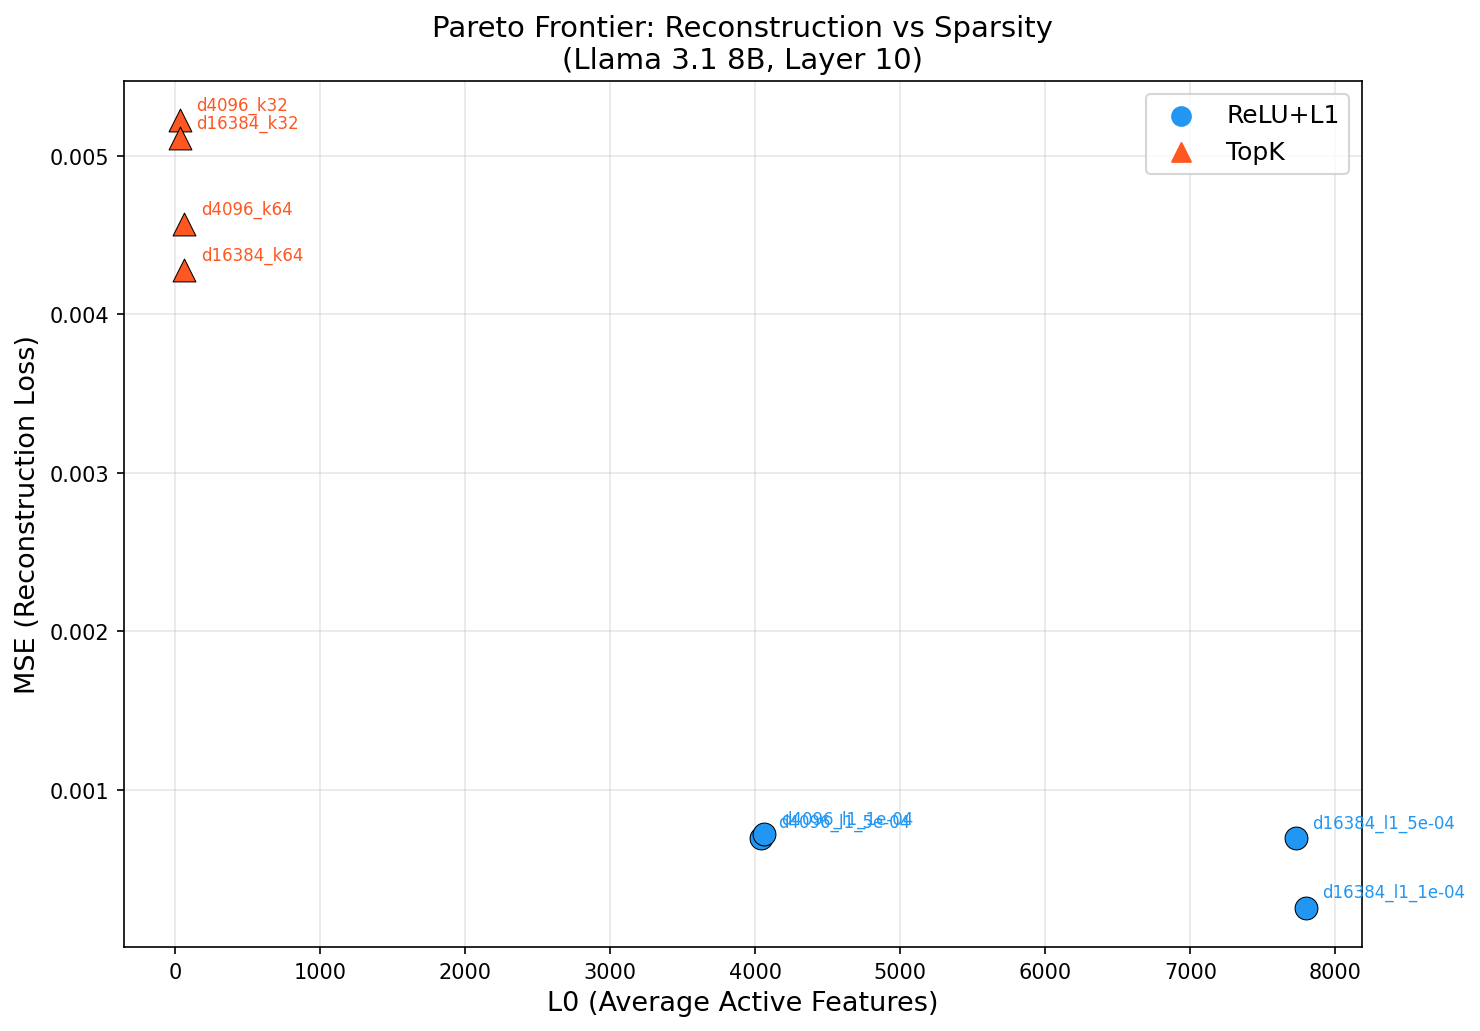
\includegraphics[width=\textwidth]{figures/pareto_llama.png}
    \caption{Llama 3.1 8B}
\end{subfigure}
\caption{Pareto frontier: reconstruction loss (MSE) vs.\ sparsity ($\ell_0$-norm $L_0$) for all 8 SAE configurations per model. Blue circles = ReLU+L1; orange triangles = TopK.}
\label{fig:pareto}
\end{figure}

TopK performance is strongly model-dependent: 79.7\% FVE on Gemma~2B (35.3\% dead) versus 98.0\% on Llama~8B (31.3\% dead). ReLU+L1 exceeds 99\% FVE on both models with near-zero dead rates, making it the more robust choice; Section~\ref{sec:topk-gap} discusses the likely source of the gap.

\subsection{Language Probing}

Linear probing (logistic regression, 5-fold CV) on mean-pooled layer-10 activations for 5-way language classification yields near-perfect accuracy for both models (Table~\ref{tab:probing}), confirming that language identity is linearly separable in the residual stream and that SAE encoding preserves this information.

\begin{table}[t]
\centering
\caption{Language classification accuracy (5-fold CV, 1,012 samples per language). The best custom SAE (by FVE) is used for SAE feature probing.}
\label{tab:probing}
\begin{tabular}{lcc}
\toprule
\textbf{Representation} & \textbf{Gemma 2B} & \textbf{Llama 8B} \\
\midrule
Raw activations ($d_\text{model}$) & 99.94\% $\pm$ 0.12 & 99.98\% $\pm$ 0.04 \\
SAE features ($d_\text{sae}$) & 99.98\% $\pm$ 0.04 & 99.88\% $\pm$ 0.15 \\
\bottomrule
\end{tabular}
\end{table}

All accuracies exceed 99.8\%, meaning a simple linear classifier can distinguish languages from a single layer's activations. SAE features achieve comparable accuracy to raw activations despite imperfect reconstruction (FVE of 99.2\% for the Gemma SAE and 99.8\% for the Llama SAE used for probing), confirming that the SAE decomposition retains language-relevant information.

\subsection{Portuguese-Specific Features}
\label{sec:features}

Differential analysis (Eq.~\ref{eq:diff}) with pretrained SAEs identifies strongly Portuguese-specific features ($s_i > 2$) across all analyzed layers in both models (Table~\ref{tab:features}).

\begin{table}[t]
\centering
\caption{Strongly PT-specific feature counts ($s > 2$) at each analyzed layer using pretrained SAEs (column headers indicate layer indices; Gemma 2B: layers 0, 5, 10, 15, 20, 25; Llama 8B: layers 0, 5, 10, 16, 21, 26). Llama counts use padding-masked analysis. The differential activation score has a theoretical ceiling of $\sqrt{5} \approx 2.236$.}
\label{tab:features}
\begin{tabular}{lccccccc}
\toprule
\textbf{Model (SAE)} & \textbf{Layer 0} & \textbf{Layer 5} & \textbf{Layer 10} & \textbf{Layer 15/16} & \textbf{Layer 20/21} & \textbf{Layer 25/26} & \textbf{Total} \\
\midrule
Gemma 2B (16k) & 625 & 320 & 402 & 263 & 253 & 460 & 2,323 \\
Llama 8B (32k) & 698 & 675 & 747 & 646 & 593 & 452 & 3,811 \\
\bottomrule
\end{tabular}
\end{table}

Both models contain thousands of strongly PT-specific features distributed across all layers. Normalizing for SAE dictionary size yields comparable densities: Gemma has 2,323/16,384 = 14.2\%, while Llama has 3,811/32,768 = 11.6\%. The layer-wise distributions differ. Gemma~2B concentrates features at layers~0 (625) and~25 (460), the input and output boundaries, while Llama~8B shows a monotonic decrease from layer~0 (698) to layer~26 (452), suggesting that language-specific information is most prominent in early layers and is progressively absorbed into more abstract representations.

From the set of strongly PT-specific features in Gemma~2B we selected the top 20 features per layer by differential score, yielding 120 features across the 6 analyzed layers. Manual inspection of their top-activating tokens reveals interpretable categories (Table~\ref{tab:feature_categories}).

\begin{table}[t]
\centering
\caption{Categories of Portuguese-specific features in Gemma~2B (120 features across 6 layers, categorized by top-activating tokens).}
\label{tab:feature_categories}
\begin{tabular}{llll}
\toprule
\textbf{Category} & \textbf{Count} & \textbf{Example tokens} & \textbf{Dominant layers} \\
\midrule
Morphological & 24 & ``-\c{c}\~ao'', ``-sivo'', ``\^enio'' & layers 5--15 \\
Syntactic & 18 & ``do'', ``pelo'', ``em'', ``uma'' & layer 0, layers 20--25 \\
Lexical & 4 & ``Maia'', ``Oliveira'' & layers 15--25 \\
Semantic & 1 & ``brasileiro'' & layer 15 \\
Shared Romance & 1 & (active for multiple langs) & layer 10 \\
Unclassified & 72 & (no clear dominant token) & all \\
\bottomrule
\end{tabular}
\end{table}

A layer-wise gradient emerges: the earliest layer (layer 0) predominantly captures syntactic features (function words, articles), middle layers (layers 5--15) capture morphological patterns (Portuguese-specific suffixes), and later layers (layers 20--25) capture more complex syntactic constructions (contractions, preposition usage).

For Llama~8B, many top features initially activated on padding tokens, an artifact of differential tokenization lengths (PT averages 40.5 tokens/sentence vs.\ EN's 27.8). Masking padding positions before computing mean activations reduces the strongly PT-specific count from 4,143 to 3,811 ($-8\%$); Table~\ref{tab:llama_features} shows the corrected top-20.

\begin{table}[t]
\centering
\caption{Top-20 Llama-Scope PT features (layer 10) after padding masking. Features are categorized by their top-activating tokens on genuine (non-padding) Portuguese text.}
\label{tab:llama_features}
\footnotesize
\begin{tabular}{lllp{5cm}}
\toprule
\textbf{Category} & \textbf{Count} & \textbf{Example tokens} & \textbf{Note} \\
\midrule
Syntactic & 14 & ``de'', ``os'', ``a'', ``um'', ``que'', ``com'' & Prepositions, articles, conjunctions \\
Morphological & 4 & ``s\~ao'', ``\^a'', ``-icos'', ``-ode'' & PT verb forms, suffixes \\
Mixed/subword & 2 & ``ab'', ``di'' & Subword fragments in PT contexts \\
\bottomrule
\end{tabular}
\end{table}

We restricted manual inspection to the top-20 features at the SAE-training layer (layer 10) for Llama, against 120 features across all 6 analyzed layers for Gemma, reflecting the cost of token-level inspection of Llama-Scope's larger dictionary. After masking, syntactic features (prepositions ``de''/``com'', articles ``a''/``os''/``um'') dominate, with morphological features (``s\~ao'', ``\^a'', suffixes ``-icos'') also present---mirroring Gemma's layer-10 composition. Methodologically, differential analysis on padded sequences can produce spurious results when languages tokenize to different lengths, a pitfall we are not aware of having been documented in the SAE interpretability literature.

\subsection{Steering Results}
\label{sec:steering}

Our central result is the divergent fallback behavior produced by suppression, illustrated in Table~\ref{tab:steering}.

\begin{table}[t]
\centering
\caption{Steering examples. \emph{Baseline}: normal generation; \emph{Suppression}: top-20 PT features set to zero; \emph{Amplification}: top-20 PT features multiplied by 10. Fallback-language labels (\textbf{in bold}) were assigned by manual inspection of the generated text.}
\label{tab:steering}
\footnotesize
\begin{tabular}{p{2.0cm}lp{4.2cm}p{4.2cm}}
\toprule
\textbf{Prompt} & \textbf{Mode} & \textbf{Gemma 2B output} & \textbf{Llama 8B output} \\
\midrule
\multirow{3}{2.0cm}{\raggedright\emph{A capital do Brasil \'e}} & Base & palco de diversos eventos e festivais... & o centro mais importante do pa\'is... \\
\cmidrule{2-4}
 & Suppr. & la una metr\`opolis ambduna de les fa uns centenars... \textbf{(Catalan)} & a capital, 1 capital, is 1 capital... \textbf{(English)} \\
\cmidrule{2-4}
 & Amplif. & uma das m\'etroas mais importantes da metropode... \textbf{(PT, degraded)} & que que que u u u... \textbf{(collapsed)} \\
\midrule
\multirow{2}{2.0cm}{\raggedright\emph{O rio mais longo do mundo \'e}} & Suppr. & el f\'erriable del continente... \textbf{(Spanish)} & the longest the most long the... \textbf{(English)} \\
\cmidrule{2-4}
 & Amplif. & o Brasil, e sua extens\~ao \'e de 235 mil quil\^ometros... \textbf{(PT)} & mais do mais mais... \textbf{(collapsed)} \\
\midrule
\multirow{2}{2.0cm}{\raggedright\emph{A l\'ingua portuguesa \'e falada em}} & Base & 22 pa\'ises, sendo Portugal um dos principais... & mais de 70 pa\'ises, cerca de 200 milh\~oes de falantes... \\
\cmidrule{2-4}
 & Suppr. & todos os continentes, enrapapeando la lengua espa\~nola... \textbf{(Spanish)} & il...?...?...? \textbf{(degenerate)} \\
\bottomrule
\end{tabular}
\end{table}

\noindent The third prompt was not included in the factor-10 amplification batch; it appears here to illustrate that Gemma's Spanish fallback preserves topical coherence (see Section~\ref{sec:discussion}).

\paragraph{Gemma 2B: Romance-Language Continuum.} Suppressing Portuguese features consistently redirects generation to Spanish or Catalan, closely related Romance languages. The model appears to organize languages in a continuous space where typologically related languages are neighbors; removing Portuguese-specific features causes the model to fall back to the nearest Romance representation. In the third example, the Portuguese prompt about the Portuguese language continues in Spanish with thematically related content.

\paragraph{Llama 8B: English Substrate.} Suppressing Portuguese features redirects generation to English. This aligns with the ``English pivot'' hypothesis of Wendler et al.~\cite{wendler2024llamas}: Llama models appear to build non-English representations as language-specific overlays on top of English-centric features. Stripping the Portuguese overlay reveals the underlying English default.

\paragraph{Amplification.} In Gemma~2B, factor-10 amplification produces Portuguese output with morphological degradation but preserved language identity. In Llama~8B, the same factor causes textual collapse (Figure~\ref{fig:steering_comparison}). Lower factors (2--3) on Llama yield intermediate results: factor-2 produces repetitive but recognizably Romance-influenced output, and at factor~3 the top-ranked PT-specific feature (feature~2142 in Llama-Scope layer 10) generates ``trabalho do'' (``work of''). The asymmetry may reflect Llama-Scope's 32k JumpReLU features producing larger individual activations than Gemma Scope's ReLU features, which would make multiplicative amplification disproportionately disruptive; a direct magnitude comparison is left to future work.

\begin{figure}[t]
\centering
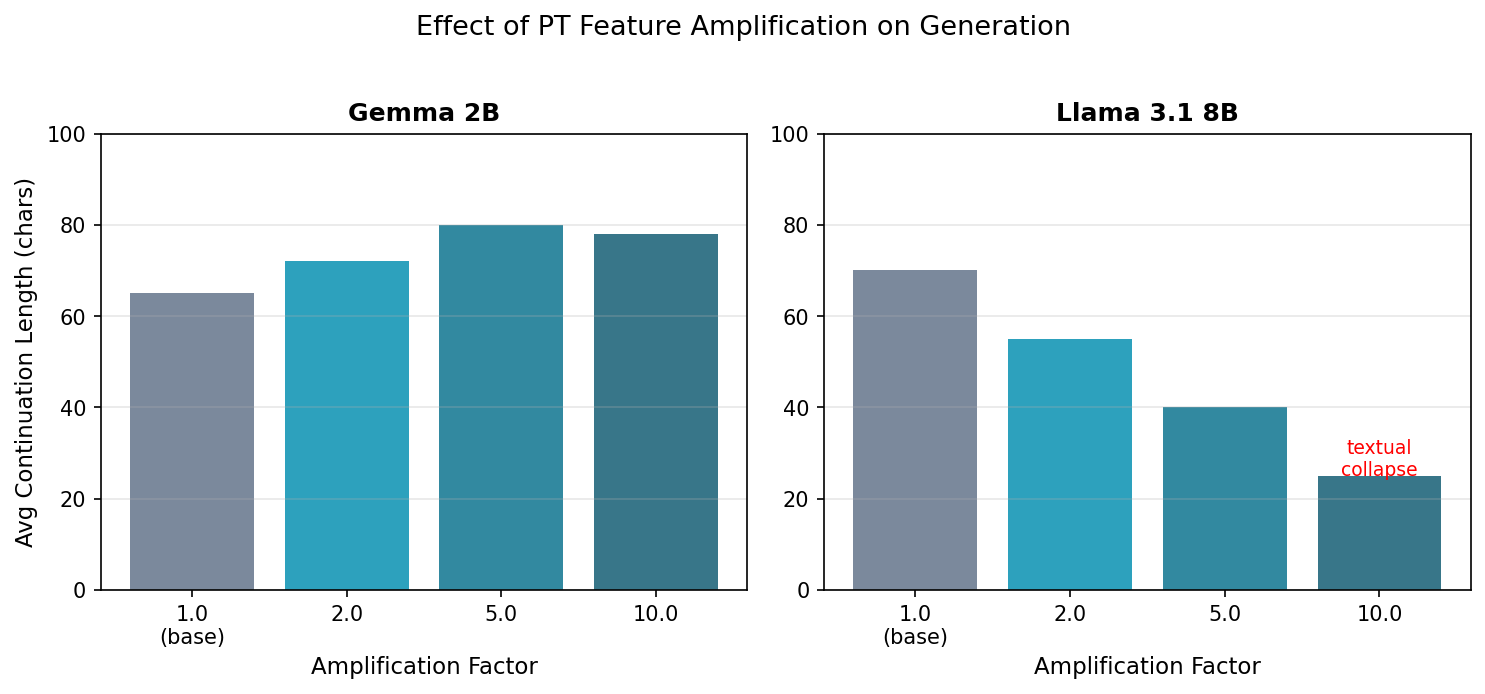
\includegraphics[width=0.85\textwidth]{figures/steering_comparison.png}
\caption{Effect of PT feature amplification on generation across models. Gemma~2B maintains generation coherence at high amplification factors, while Llama~8B exhibits progressive textual collapse.}
\label{fig:steering_comparison}
\end{figure}

\paragraph{Individual Feature Analysis.}
Amplifying individual features in Llama~8B (factor 5.0, baseline ``uma das capitais brasileiras mais belas...'' from prompt \emph{``A capital do Brasil \'e''}) reveals interpretable specializations. Feature~16811 produces repetitions exclusively from \{Portugal, Portuguese, Brazil\}, suggesting a ``Lusophone world'' concept; feature~18397 generates a PT-EN hybrid (\emph{``a capital do Brazil is the capital of Britain countries''}), functioning as a cross-lingual bridge; feature~16096 yields Brazil-anchored repetitions (\emph{``BC Brazil is BC Brazil is is is...''}).

\paragraph{Progressive Multi-Layer Steering.}
To localize language identity, we performed progressive steering on Gemma~2B, amplifying the top-20 PT-specific Gemma Scope features (factor~5) at an increasing number of layers. Each continuation is scored by a \emph{PT-likeness} heuristic $0.3\,c + 10\,w$, where $c$ counts Portuguese-specific characters (``\~a'', ``\c{c}'', ``\^a''\dots) and $w$ is the ratio of common Portuguese function words (``de'', ``do'', ``que''\dots); this is distinct from the differential activation score of Eq.~\ref{eq:diff}. On continuations where a published LID assigns PT confidence above 0.1 ($n{=}55$), PT-likeness and fastText LID-176~\cite{joulin2016bag} show Spearman $\rho{=}0.83$; published LIDs themselves report near-zero PT probability on the degenerate outputs of this experiment (median fastText PT probability 0.003 across 147 steering continuations), so marker counting is the appropriate signal here. Steering layer~25 alone yields PT-likeness 4.5; adding layer~20 drops it to 2.55 (interference); 15+20+25 together yields 7.2, with Portuguese function words and diacritics in the output; adding layer~10 drops it to 0.9 (incoherent text). Language identity is therefore encoded in mid-to-late layers (15--25), and steering early layers disrupts foundational representations the later layers depend on, which also explains why our multi-layer steering (Table~\ref{tab:steering}) succeeds where single-layer steering does not.

\subsection{Cross-Scale Analysis}
\label{sec:crossscale}

To disentangle family effects from scale effects, we also analyzed Gemma-2-9B (42 layers, $d_\text{model}=3{,}584$) using raw neuron activations (Table~\ref{tab:crossscale}).

\begin{table}[t]
\centering
\caption{Cross-scale comparison within the Gemma family. Cosine similarity between mean PT and ES/EN activations, and count of strongly PT-specific neurons ($s > 2$, where $s$ is the differential activation score of Eq.~\ref{eq:diff} applied to raw neurons rather than SAE features).}
\label{tab:crossscale}
\begin{tabular}{ccccc}
\toprule
\textbf{9B Layer} & \textbf{Rel.\ pos.} & \textbf{cos(PT,ES)} & \textbf{cos(PT,EN)} & \textbf{$n_{s>2}$} \\
\midrule
0  & 0\% & 0.9998 & 0.9995 & 9 \\
8  & 20\% & 0.9996 & 0.9990 & 18 \\
16 & 39\% & 0.9998 & 0.9995 & 11 \\
24 & 59\% & 0.9995 & 0.9990 & 25 \\
32 & 78\% & 0.9983 & 0.9966 & 22 \\
\textbf{41} & \textbf{100\%} & \textbf{0.9883} & \textbf{0.9815} & \textbf{41} \\
\bottomrule
\end{tabular}
\end{table}

The 9B model shows progressive linguistic differentiation (Figure~\ref{fig:crossscale}): cosine similarity between Portuguese and Spanish mean activations drops monotonically from 0.9998 (layer 0) to 0.9883 (layer 41). The PT-EN drop is steeper still (0.9995 $\to$ 0.9815). The number of strongly PT-specific neurons increases from 9 (layer 0) to 41 (layer 41). The 2B model, by contrast, shows top differential activation scores pinned near the theoretical ceiling at every analyzed layer (all $\sim$2.236, the value of $\sqrt{5}$). We rely on the qualitative contrast (flat vs progressive) rather than absolute magnitudes, since the 2B and 9B numbers live in different spaces: 2B scores are computed on Gemma Scope SAE features, while 9B scores use raw neuron activations because no pretrained SAE suite was available for the 9B model at the time of this study. The pattern suggests that larger models develop finer language separation in deeper layers, a property not visible at the 2B scale.

\begin{figure}[t]
\centering
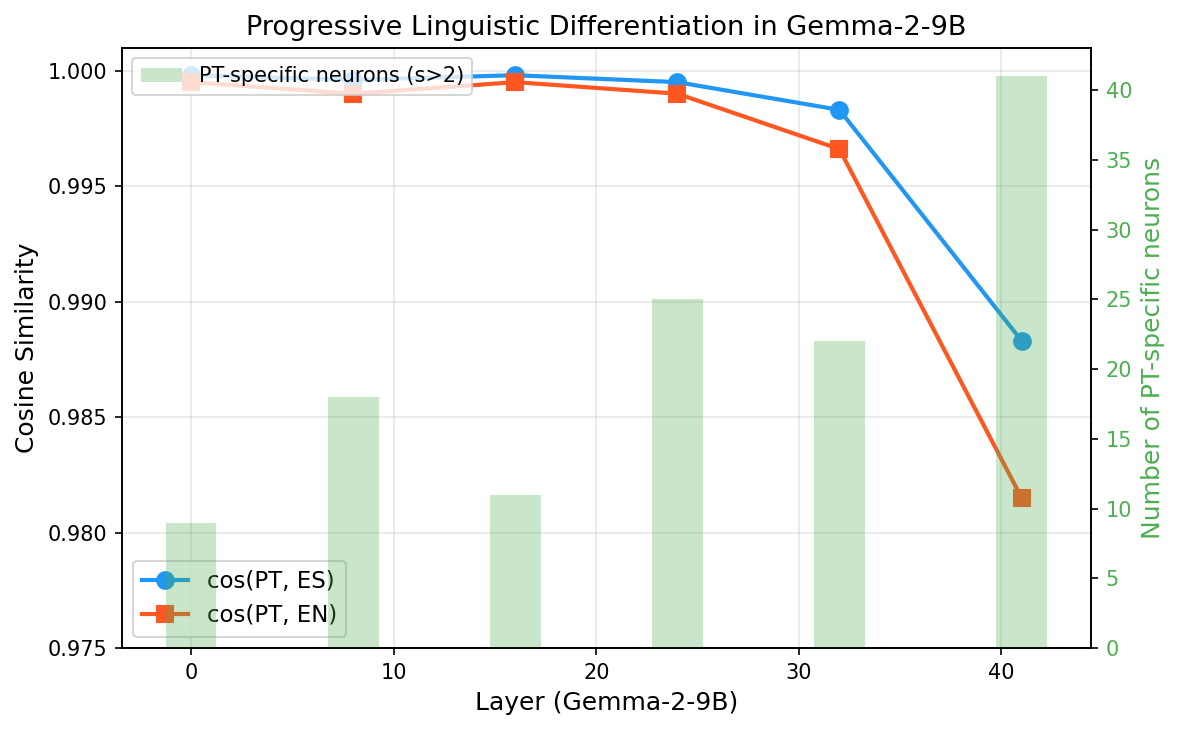
\includegraphics[width=0.75\textwidth]{figures/crossscale_similarity.png}
\caption{Progressive linguistic differentiation in Gemma-2-9B: cosine similarity between Portuguese and Spanish/English mean activations decreases in deeper layers, while the number of PT-specific neurons increases. This gradient is absent in the 2B model.}
\label{fig:crossscale}
\end{figure}

% ============================================================
\section{Discussion}
\label{sec:discussion}

\subsection{Cross-Family Language Organization}

Our central finding, divergent fallback languages upon feature suppression, suggests two distinct paradigms for multilingual representation. We hypothesize that these differences stem primarily from training data composition. A pairwise cosine similarity analysis on mean FLORES activations across layers supports a layered separation: in both models, PT-EN distance (Romance vs.\ Germanic) is largest from the earliest layers, PT-FR distance (cross-subfamily) grows in middle layers, and PT-ES distance (Iberian) only diverges in late layers. For Gemma~2B at layer~25 we measure cos(PT,ES)$=0.958$, cos(PT,FR)$=0.928$, cos(PT,EN)$=0.932$, computed on the same mean-pooled FLORES activations used for the cross-scale analysis of Table~\ref{tab:crossscale}. This ordering reflects typological distance and suggests that the continuum has variable granularity across depth.

The Romance-language continuum observed in Gemma~2B organizes languages descended from Latin in a representational space where typological proximity maps to representational proximity. When Portuguese features are suppressed, \emph{``A l\'ingua portuguesa \'e falada em''} continues coherently in Spanish (\emph{``todos os continentes, enrapapeando la lengua espa\~nola...''}) and switches topic to language distribution. In another example the fallback drifts into Catalan (\emph{``la una metr\`opolis ambduna de les fa uns centenars''}), a language absent from our five FLORES evaluation languages, indicating that the continuum is not merely a ranking over the measured set but a broader typological geometry that includes Romance varieties we did not evaluate. Gemma is trained on curated multilingual data with deliberate language balancing~\cite{lieberum2024gemma}, which may encourage the model to learn shared Romance structure rather than treating each language independently.

In Llama~8B the pattern is different. The same suppression experiment on ``O rio mais longo do mundo \'e'' produces \emph{``the longest the most long the is the more long the''}, a degraded but recognizably English translation of the prompt's meaning. This is consistent with Wendler et al.~\cite{wendler2024llamas}'s finding that Llama~2 uses English as an internal \emph{lingua franca}: non-English inputs are processed through English-centric intermediate representations. Meta's Llama models are trained on predominantly English data (${\sim}90\%$ English in the Llama 2 pretraining mix~\cite[Table~10]{touvron2023llama2}), which would naturally lead to English as the ``base layer'' upon which other language capabilities are added.

To quantify this contrast, we apply the monolinguality metric of Eq.~\ref{eq:monolinguality} to PT-dominant neurons. Averaged across the analyzed layers, Llama~8B has higher mean PT monolinguality (0.270) than Gemma~2B (0.252), and the gap widens in later layers (Llama reaches 0.35 at layer~31 vs.\ Gemma's 0.28 at layer~25). This confirms that the English substrate in Llama produces sharper language boundaries, while Gemma's Romance continuum creates more diffuse, shared representations. The Llama depth pattern is internally consistent: PT-specific feature counts in Table~\ref{tab:features} decrease from layer 0 (698) to layer 26 (452), while PT monolinguality rises from earlier layers to 0.35 at layer 31. The two trends together describe a progression toward fewer but more sharply PT-specific features in deeper layers, rather than a contradiction. The feature-category distributions in Tables~\ref{tab:feature_categories} and~\ref{tab:llama_features} echo the same contrast: Gemma's 120 layer-spanning features include a ``Shared Romance'' category with cross-Romance activation, while Llama's top-20 at layer 10 include mixed/subword fragments and, under individual steering, a PT-EN bridge feature~(18397)---different flavors of cross-language sharing that match the continuum and substrate paradigms.

The PT-EN bridge feature~18397 (Section~\ref{sec:steering}) has no analogue in Gemma, consistent with the continuum picture where Romance languages share representational space rather than translating across layers. Our suppression experiments can also be viewed as intentionally induced code-switching, connecting to SASFT~\cite{sasft2026}; the Romance fallback in Gemma is consistent with their finding that code-switching is triggered by elevated pre-activation values of neighboring language features.

These two paradigms have practical implications. The Romance-language continuum may allow finer-grained language steering by ``sliding'' between related languages, while the English substrate raises concerns about English-centric biases propagating to all other languages. More broadly, our findings suggest that training data proportions shape internal language architecture, not just downstream performance.

\subsection{TopK Performance Across Models}
\label{sec:topk-gap}

The TopK gap (79.7\% FVE on Gemma~2B vs.\ 98.0\% on Llama~8B) appears under identical hyperparameters. A plausible explanation is activation intrinsic dimensionality: Llama's $d_\text{model}{=}4{,}096$ (nearly twice Gemma's 2,304) offers a higher-dimensional space where activations may concentrate on a $k$-sparse basis more readily, while Gemma's lower-dimensional activations diffuse across many components and defeat exact-$k$ sparsity. ReLU+L1 adapts its sparsity per sample and exceeds 99\% FVE on both models; TopK produces $\sim$35\% dead features on both, versus $<$1.2\% for ReLU+L1. The practical takeaway is that TopK transfer is not automatic: practitioners should validate on their specific base model.

\subsection{Limitations}
\label{sec:limitations}

Our two models differ simultaneously in family, size, attention variant, and training mix, so the observed differences in fallback behavior may reflect any combination of these factors; the within-family 2B vs.\ 9B analysis mitigates only scale effects, and a fully controlled comparison would require same-size models from different families. The pretrained SAEs themselves differ in activation function, dictionary size, and training procedure, so we rely on qualitative contrasts (fallback language, feature categories) rather than absolute counts, and normalize by dictionary size where counts are reported. On the steering side, factor-10 amplification collapses Llama output and layer-10 steering disrupts the foundational representations that later layers depend on (Section~\ref{sec:steering}); recent work~\cite{causal_lang_control2025} shows $90\%$ single-feature steering between typologically distant languages, indicating that the difficulty we observe within Romance languages reflects genuinely shared representations rather than a methodological wall. Finally, steering generation uses temperature $T{=}0.7$, so the specific strings in Table~\ref{tab:steering} are illustrative; the qualitative conclusions (fallback identity, feature categories) are stable across prompts and runs.

In scope, we analyze 6 of 26--32 layers per model, 5 European languages (4 Romance), and a single corpus (FLORES-200); the European focus may inflate Portuguese specificity scores and other genres may activate different features. 60\% of Gemma's 120 inspected features remain unclassified; automated LLM-based interpretation could improve coverage but introduces its own biases. Future work should extend to additional model families (Mistral, Qwen) and to same-size comparisons, include typologically diverse languages, and investigate PT-BR vs.\ PT-PT dialect variation.

% ============================================================
\section{Conclusion}

We presented a cross-family mechanistic interpretability study of Portuguese representation in Gemma-2-2B and Llama~3.1~8B. Sparse autoencoders identify Portuguese-specific features in both models, and steering experiments establish their causal role. Suppressing Portuguese features produces an English fallback in Llama and a Romance-language fallback in Gemma, revealing two paradigms that we term the ``English substrate'' and ``Romance-language continuum'' models. A monolinguality metric on raw neurons quantifies the contrast (0.270 in Llama vs.\ 0.252 in Gemma), progressive multi-layer steering localizes language identity to mid-to-late layers (15--25), and pairwise similarity analysis shows that typological distance is encoded from the earliest layers.

\paragraph{Reproducibility.} Code, trained SAE checkpoints, extracted activations, and experimental results are available at \url{https://anonymous.4open.science/r/llm-pt-interpretability-EC0D/}\footnote{Anonymous repository for double-blind review; the non-anonymous version will be released upon acceptance.}.

% ============================================================
\bibliographystyle{splncs04}
\bibliography{references}

\end{document}
